
\de{ĐỀ THI HỌC KỲ I NĂM HỌC 2022-2023}{THPT Thực Hành Sài Gòn}


\begin{bt}%[0T3B1-2]%[0T3B1-4]%[Dự án đề kiểm tra HKII NH22-23- Nguyễn Ngọc Nguyên]%[Trường Trung Học Thực Hành Sài Gòn]
	\begin{enumerate}
	\item Tìm tập xác định của hàm số sau $y=f(x)=\sqrt{3x+2}$.
	\item Tìm các khoảng đồng biến, nghịch biến của hàm số có đồ thị như sau:
	\begin{center}
		\begin{tikzpicture}[>=stealth,x=1cm,y=1cm,scale=1, font=\normalsize]
			\def\a{1} 
			\def\b{-4}
			\def\c{3}
			\draw[line width=1,->] (-2,0) -- (11,0) node[below] {$x$};
			\draw[line width=1,->] (0,-2) -- (0,5) node[left] {$y$};
			\draw (0,0)node[below left]{$O$};
			\draw[thick,samples=150,smooth,domain=0:4] plot(\x,{\a*(\x)^2+(\b)*\x+(\c)}) ;
			\draw[thick] (4,3)--(10,0);
			\foreach \x in {-1,1,3,4,5,...,10} \draw[line width=0.75] (\x,0.1)--(\x,-0.1) node [below] {$\x$} ;
			\draw[line width=0.75] (2,-0.1)--(2,0.1) node [above] {$2$} ;
			\foreach \y in {-1,1,2,3,4}\draw[line width=0.75] (0.1,\y)--(-0.1,\y) node [left] {$\y$}; 
			\draw[dashed] (2,0)|-(0,-1) (4,0)|-(0,3);
		\end{tikzpicture}
	\end{center}
	\end{enumerate}
	\dapso{a) $D=\left[ \dfrac{-2}{3};+\infty \right) $; b) $f(x)$ đồng biến trên $(2;4)$ và nghịch biến trên $(0;2)$ và $ (4;10)$.}
	\loigiai{
		\begin{enumerate}
			\item Điều kiện xác định: $3x+2 \ge 0 \Leftrightarrow x \ge -\dfrac{2}{3}$.\\
			Vậy tập xác định của hàm số là $\mathscr{D}=\left[- \dfrac{2}{3};+\infty \right)$.
			\item Từ hình vẽ ta thấy đồ thị hàm số đi lên trên khoảng $(2;4)$ nên hàm số đồng biến trên khoảng $(2;4)$.\\
			Đồ thị hàm số đi xuống trong khoảng $(0;2)$ và $(4;10)$ nên hàm số nghịch biến trên khoảng $(0;2)$ và $(4;10)$. 
		\end{enumerate}
	}
\end{bt} 

\begin{bt}%[0T3B2-1]%[0T3B2-3][Dự án đề kiểm tra HKII NH22-23- Nguyễn Ngọc Nguyên]%[Trường Trung Học Thực Hành Sài Gòn]
	Lập bảng biến thiên và vẽ đồ thị của hàm số $y=f(x)=-x^2+5x-4$.
	\loigiai{
	Tập xác định của hàm số $f(x)$ là $\mathscr{D}=\mathbb{R}$.\\
	Tọa độ đỉnh $I\left( \dfrac{5}{2};\dfrac{9}{4} \right)$.\\
	Trục đối xứng $x=\dfrac{5}{2}$.\\
	Hệ số $a=-1<0$ nên bề lõm của parabol hướng xuống dưới.\\
	Cho $f(x)=0 \Leftrightarrow \hoac{&x=1 \\ &x=4}$. Suy ra đồ thị hàm số cắt trục $Ox$ tại hai điểm có tọa độ $(1;0)$ và $(4;0)$. \\
	Cho $x=0 \Rightarrow f(0)=-4$. Suy ra đồ thị hàm số cắt trục $Oy$ tại điểm có tọa độ $(0;-4)$. \\
	Ta có bảng biến thiên và đồ thị như hình vẽ.
\begin{multicols}{2}
	
\begin{tikzpicture}[scale=1, font=\footnotesize,line join=round, line cap=round,>=stealth]
		\tkzTabInit[nocadre=false,lgt=1.2,espcl=2.5,deltacl=0.6]{$x$/0.8,$f(x)$/2}
		{$-\infty$,$\dfrac{5}{2}$,$+\infty$}
		\tkzTabVar{-/$-\infty$,+/$\dfrac{9}{4}$,-/$-\infty$}
	\end{tikzpicture}	
\begin{tikzpicture}[scale=0.85,>=stealth, font=\footnotesize, line join=round, line cap=round]
	\draw[->] (-1,0)--(6,0) node [below]{$x$};
	\draw[->] (0,-5)--(0,3) node [left]{$y$};
	\node at (0,0) [below left]{$O$};
	\clip (-1,-4.2) rectangle (6,3);
	\draw[smooth,samples=300,domain=-0.5:5] plot(\x,{-1*(\x)^2 +5*(\x) -4});
	\draw (1,0) node[below right] {$1$} (4,0) node[below left] {$4$} (0,-4) node[left] {$-4$}; 
	\draw[dashed] (2.5,0) node[below] {$\dfrac{5}{2}$} -- (2.5,2.25) --(0,2.25) node[left] {$\dfrac{9}{4}$};
\end{tikzpicture}
\end{multicols}
	}
\end{bt}

\begin{bt}%[0T3K2-5]%[Dự án đề kiểm tra HKII NH22-23- Nguyễn Ngọc Nguyên]%[Trường Trung Học Thực Hành Sài Gòn]
	Trong hình vẽ minh họa bên dưới, một vận động viên bóng chuyền đứng cách phía sau vạch quy định $1$ m đang tập phát bóng. Độ cao $h$ (m) của quả bóng sau thời gian $t$ giây tính từ lúc bắt đầu phát bóng được cho bởi hàm số $h=-4{,}9t^2+3{,}82t+1{,}7$.
	\begin{center}
\definecolor{battleshipgrey}{rgb}{0.52, 0.52, 0.51}

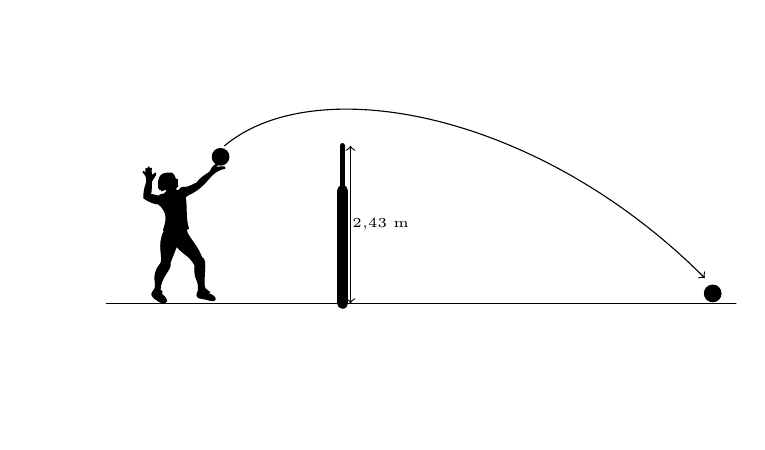
\begin{tikzpicture}[line join=round, line cap=round,scale=1,transform shape]
	\clip (-4,-2.5) rectangle (5,2.5);
	\tikzset{vdv/.pic={
			\def\T{ 
				(-.4,1.55)
				..controls +(175:.3) and +(95:.4) ..  (-.8,1.1)--(-.76,1.12)--(-.77,1.06)--(-.7,1.08)--(-.72,1.02)--(-.62,1.06)
				..controls +(-15:.15) and +(45:.15) ..  (-.64,.92)
				..controls +(175:.1) and +(-155:.05) ..  (-.8,.85)
				..controls +(155:.05) and +(15:.05) .. (-1.05,.9)
				..controls +(75:.1) and +(-85:.05) .. (-1.02,1.3)
				..controls +(45:.1) and +(-145:.05) .. (-.9,1.5)
				..controls +(75:.15) and +(35:0) .. (-.97,1.48)
				..controls +(165:.1) and +(-90:0) .. (-1.02,1.7)
				..controls +(145:.07) and +(75:0) .. (-1.07,1.55)
				..controls +(115:.05) and +(-85:0) .. (-1.09,1.74)
				..controls +(145:.07) and +(-90:0) .. (-1.12,1.54)
				..controls +(115:.05) and +(-85:0) .. (-1.16,1.69)
				..controls +(145:.07) and +(-90:0) .. (-1.17,1.53)
				..controls +(135:.05) and +(-85:0) .. (-1.26,1.6)
				..controls +(-145:.08) and +(90:.3) .. (-1.16,1.3)
				..controls +(-95:.08) and +(90:.3) .. (-1.25,.8)
				..controls +(-25:.05) and +(175:.25) .. (-.8,.62)
				..controls +(-40:.5) and +(85:.15) .. (-.65,-.18)--(-.62,-.18)
				..controls +(-120:.5) and +(50:.2) .. (-.75,-1.2)
				..controls +(-130:.5) and +(50:.25) .. (-.95,-2)
				..controls +(-130:.1) and +(150:.3) .. (-.82,-2.3)
				..controls +(-60:.1) and +(-40:.5) .. (-.72,-2.1)
				..controls +(70:.1) and +(-40:.1) .. (-.76,-1.98)
				..controls +(90:.4) and +(-70:.2) .. (-.46,-1.16)--(-.26,-.65)
				..controls +(-50:.4) and +(120:.4) .. (.3,-1.23)
				..controls +(-95:.5) and +(85:.4) .. (.4,-2)
				..controls +(-115:.3) and +(165:.2) .. (.65,-2.26)
				..controls +(-20:.4) and +(-10:.25) .. (.7,-2.1)--(.74,-2.05)--(.6,-1.94)
				..controls +(120:.2) and +(-10:.2) .. (.5,-1)
				..controls +(110:.45) and +(-120:0.15) .. (.05,-.14)--(.1,-.12)
				..controls +(110:.3) and +(-70:0.15) .. (0,.8)
				..controls +(70:.05) and +(-170:0.05) .. (.1,.9)
				..controls +(25:.7) and +(-170:0.5) .. (1.2,1.7)
				..controls +(70:.1) and +(-20:0.1) .. (.92,1.74)
				..controls +(120:.05) and +(-120:0.05) .. (.98,1.8)
				..controls +(120:.05) and +(70:0.2) .. (.76,1.6)
				..controls +(-120:.05) and +(55:0.25) .. (.35,1.25)
				..controls +(170:.05) and +(-5:0.25) .. (-.1,1.12)
				..controls +(-170:.02) and +(45:0.05) .. (-.2,1.02)--(-.28,1.04)--(-.29,1.1)
				..controls +(20:.15) and +(-130:0.08) .. (-.23,1.35)
				..controls +(160:.17) and +(-45:0.25) .. cycle
				;}
			\draw \T;
			\fill \T;
	}}
	\draw (-3,-1)--(5,-1);
	\draw[fill=black] (-1.55,.86) circle (3pt);
	\draw[fill=black] (4.7,-.875) circle (3pt);
	\node at (0,0) [right]{\tiny $2{,}43$ m};
	\draw[line width=4] (0,.43)--(0,-1);
	\draw[line width=2] (0,.43)--(0,1);
	\draw[<->] (0.1,1)--(0.1,-1);
	\draw[->] (-1.5,1)..controls +(40:1.5) and +(135:3) ..  (4.6,-.68);
	\path (-2,0)pic[scale=.42]{vdv}
	;
\end{tikzpicture}
	\end{center}
	\begin{enumerate}
		\item Khi nào quả bóng đạt được độ cao cao nhất (làm tròn kết quả đến chữ số thập phân thứ hai)?
		\item Quả bóng đến lưới lúc $t=0{,}6$ giây. Liệu bóng có qua lưới không? Hãy giải thích, biết chiều cao lưới là $2{,}43$ m
		(làm tròn kết quả đến hàng phần trăm).	
	\end{enumerate}
	\dapso{ a) $0{,}39$ giây; b) $h(0,6)=2{,}228 < 2{,}43$ nên bóng không qua lưới.}
	\loigiai{
	\begin{enumerate}
		\item 
		Quả bóng đạt được độ cao cao nhất khi $h$ có giá trị lớn nhất.\\
		Xét $h(t)=-4{,}9t^2+3{,}82t+1{,}7$ là hàm số bậc hai có bảng biến thiên như sau
		\begin{center}
		
\begin{tikzpicture}[scale=1, font=\footnotesize,line join=round, line cap=round,>=stealth]
		\tkzTabInit[nocadre=false,lgt=1.2,espcl=2.5,deltacl=0.6]{$t$/1,$h(t)$/2}
		{$0$,$\dfrac{-3{,}82}{2 \cdot (-4{,}9)}$,$\approx 1{,}096$}
		\tkzTabVar{-/$1{,}7$,+/$\approx 2{,}44$,-/$0$}
		\end{tikzpicture}	
		\end{center}
	Vậy $h(t)$ đạt giá trị lớn nhất khi $t=\dfrac{-3{,}82}{2 \cdot (-4{,}9)} \approx 0{,}39$ giây.
		\item Tại $t=0{,}6$ giây, quả bóng đạt độ cao là $h(0{,}6) =2{,}228$ m. Mà chiều cao của lưới là $2{,}43 >2{,}228$. Do đó quả bóng không qua lưới.
	\end{enumerate}
		
	}
\end{bt}



\begin{bt}%[0D5K3-2]%[Dự án đề kiểm tra HKI NH22-23- Thành Lê]%[Thực hành Sài Gòn]
	Một vận động viên $A$ tham gia tập luyện chạy cự ly $100$ mét. Kết quả sau $20$ ngày luyện tập được trình bày theo bảng dưới đây: 
	\begin{center}
		\begin{tabular}{|c|c|c|c|c|c|c|c|c|c|}
			\hline
			\multicolumn{10}{|c|}{Thời gian chạy $20$ ngày của vận động viên $A$} \\
			\hline
			$14$ & $13$ & $12$ & $15$ & $12$ & $15$ & $16$ & $14$ & $12$ & $18$ \\
			\hline
			$13$ & $16$ & $12$ & $15$ & $16$ & $14$ & $12$ & $30$ & $28$ & $13$ \\
			\hline
		\end{tabular}
	\end{center}
	\begin{enumerate}
		\item Tìm số trung bình, tứ phân vị và mốt của mẫu số liệu trên.
		\item Huấn luyện viên muốn gửi bài báo cáo thành tích cho ban huấn luyện. Trong các tham số trên, huấn luyện viên chọn tham số nào để phản ánh đúng khả năng của vận động viên $A$? Giải thích.
	\end{enumerate} 
	\dapso{ a) $\overline{x}=15{,}5$; $Q_1=12{,}5$; $Q_2=14$; $Q_3=16$; $M_0=12$; b) Số trung bình.}
	\loigiai{
		\begin{enumerate}
			\item $\overline{x}=\dfrac{12\cdot5+13\cdot3+14\cdot3+15\cdot3+16\cdot3+18+28+30}{20}=15{,}5$.\\
			Sắp xếp giá trị theo thứ tự tăng dần, ta có
			\[
			12;\ 12;\ 12;\ 12;\ 12;\ 13;\ 13;\ 13;\ 14;\ 14;\ 14;\ 15;\ 15;\ 15;\ 16;\ 16;\ 16;\ 18;\ 28;\ 30.
			\]
			Từ đó ta có $Q_2=(14+14):2=14$; $Q_1=(12+13):2=12{,}5$; $Q_3=(16+16):2=16$.\\
			Mốt của mẫu số liệu là $M_0=12$.
			\item Huấn luyện viên nên chọn \textit{Số trung bình} vì số trung bình là đại diện cho các số liệu của mẫu.
		\end{enumerate}
}
\end{bt}
\begin{bt}%[0H2G2-1]%[Dự án đề kiểm tra HKI NH22-23- Thành Lê]%[Thực hành Sài Gòn]
	Cho hình thoi $ABCD$ có $O$ là giao điểm của hai đường chéo, $AB=2a$ và $\widehat{BAD}=60^\circ$. Trên đoạn thẳng $AB$ lấy điểm $M$ sao cho $MB=2MA$. Gọi $N$ là trung điểm của đoạn thẳng $AO$. 
	\begin{enumerate}
		\item Tính tích vô hướng $\vec{AM}\cdot \vec{AN}$. 
		\item Gọi $I$ là trung điểm của đoạn thẳng $MN$. Phân tích các vectơ $\vec{AI}$, $\vec{CI}$ theo $\vec{AB}$ và $\vec{AC}$. 
		\item Đường thẳng $MN$ cắt $BC$ tại $P$. Biết $\vec{PB}=k\vec{PC}$, tìm $k$.
	\end{enumerate}
	\dapso{a) $\dfrac{1}{2}a^2$; b) $\vec{AI}=\dfrac{1}{6}\vec{AB}+\dfrac{1}{8}\vec{AC}$; $\vec{CI}=\dfrac{1}{6}\vec{AB}-\dfrac{7}{8}\vec{AC}$; c) $k=\dfrac{2}{3}$.}
	\loigiai{
		\begin{center}
			\begin{tikzpicture}[line join = round, line cap = round,>=stealth,font=\footnotesize,scale=1]
				\path
				(0,0) coordinate (A)
				(30:2.5) coordinate (B)
				(-30:2.5) coordinate (D)
				($(B)!.5!(D)$) coordinate (O)
				($(A)!2!(O)$) coordinate (C)
				($(A)!.3!(B)$) coordinate (M)
				($(A)!.5!(O)$) coordinate (N)
				($(N)!.5!(M)$) coordinate (I)
				(intersection of M--N and B--C) coordinate (P)
				($(B)!1!90:(O)$) coordinate (h)
				(intersection of P--N and B--h) coordinate (H)
				;
				\draw
				(A)--(B)--(C)--(D)--cycle (A)--(C) (B)--(D) (A)--(I) (M)--(N)--(P)--(B) (B)--(H)
				;
				\foreach \x/\g in {A/180,B/90,C/0,D/-90,O/40,M/90,N/-70,I/40,P/90,H/180} \fill (\x) circle (1.5pt) ($(\x)+(\g:3mm)$) node{$\x$};
			\end{tikzpicture}
		\end{center}
				\begin{enumerate}
				\item Ta có
				\begin{itemize}
					\item $\left|\vec{AM}\right|=AM=\dfrac{AB}{3}=\dfrac{2a}{3}$.
					\item $\triangle ABD$ đều nên $AO=\dfrac{AB\sqrt{3}}{2}=\dfrac{2a\cdot\sqrt{3}}{2}=a\sqrt{3}$.\\ 
					Vì $N$ là trung điểm của $AO
					\Rightarrow\left|\vec{AN}\right|=AN=\dfrac{AO}{2}=\dfrac{a\sqrt{3}}{2}$.
					\item $
						\vec{AM}\cdot\vec{AN}=AM\cdot AN\cdot \cos\left(\vec{AM};\vec{AN}\right)
						=\dfrac{2a}{3}\cdot\dfrac{a\sqrt{3}}{2}\cdot\cos30^\circ
						=\dfrac{a^2}{2}.
					$
				\end{itemize} 
			\item Ta có $\begin{aligned}[t]
				\vec{AI}=\vec{AM}+\vec{MI}=\vec{AM}+\dfrac{1}{2}\vec{MN}
				&=\vec{AM}+\dfrac{1}{2}\left(\vec{AN}-\vec{AM}\right)\\
				&=\dfrac{1}{2}\vec{AM}+\dfrac{1}{2}\vec{AN}\\
				&=\dfrac{1}{2}\cdot\dfrac{1}{3}\vec{AB}+\dfrac{1}{2}\cdot\dfrac{1}{4}\vec{AC}\\
				&=\dfrac{1}{6}\vec{AB}+\dfrac{1}{8}\vec{AC}.
			\end{aligned}$\\
			Ta có $
				\vec{CI}=\vec{AI}-\vec{AC}=\dfrac{1}{6}\vec{AB}+\dfrac{1}{8}\vec{AC}-\vec{AC}=\dfrac{1}{6}\vec{AB}-\dfrac{7}{8}\vec{AC}
			$.
			\item Kẻ $BH\parallel AC$ $(H\in NP)$.\\
			Ta có $BH\parallel NC\Rightarrow\dfrac{BH}{NC}=\dfrac{PB}{PC}$.\hfill$(1)$\\
			Ta có $BH\parallel NA\Rightarrow\dfrac{NA}{BH}=\dfrac{MA}{MB}$.\hfill$(2)$\\
			Nhân $(1)$ và $(2)$ vế theo vế ta có $\dfrac{NA}{NC}=\dfrac{PB}{PC}\cdot\dfrac{MA}{MB}\Rightarrow\dfrac{NC}{NA}\cdot\dfrac{PB}{PC}\cdot\dfrac{MA}{MB}=1$.\hfill$(3)$\\
			Ta có $N$ là trung điểm $AO$, $O$ là trung điểm $AC$, suy ra $\dfrac{NA}{AC}=\dfrac{1}{4}\Rightarrow\dfrac{NC}{NA}=3$.\\
			Từ $(3)\Rightarrow\dfrac{PB}{PC}\cdot\dfrac{1}{2}\cdot3=1\Rightarrow\dfrac{PB}{PC}=\dfrac{2}{3}\Rightarrow\vec{PB}=\dfrac{2}{3}\vec{PC}$.\\
			Vậy $k=\dfrac{2}{3}$.
			\end{enumerate}	
}
\end{bt}
\begin{bt}%[0D5B4-1]%[Dự án đề kiểm tra HKI NH22-23- Thành Lê]%[Thực hành Sài Gòn]
	Khi đo chiều dài của một cây cầu, các kỹ sư thu được kết quả là $\overline{a}=372{,}7362\,\text{m}\pm 0{,}001\,\text{m}$. Tìm số quy tròn của số gần đúng $372{,}7362$.
	\dapso{$a=372{,}74$.}
	\loigiai{
	Hàng lớn nhất có độ chính xác $d=0{,}001$ là hàng phần nghìn, nên ta quy tròn số đến hàng phần trăm. Vậy số quy tròn của $372{,}7362$ là $372{,}74$.
}
\end{bt}